
\documentclass[12pt,english]{article}

\usepackage[latin9]{inputenc}
\usepackage{geometry}
%\usepsackage{babel}
\usepackage{amsthm}
\usepackage{amsmath}
\usepackage{amssymb}
\usepackage{graphicx}
\usepackage{setspace}
\usepackage{hyperref}
 \usepackage{cleveref}
 \usepackage{topcapt, lscape}
 \usepackage{rotating}
 \usepackage{booktabs}
 \usepackage[para]{threeparttable}
%\usepackage{breakurl}
\usepackage{color}
\usepackage{harvard}
\usepackage{float}
\usepackage{topcapt, lscape}
%\setcounter{MaxMatrixCols}{10}
\usepackage{scalefnt}
%\usepackage{ulem}
\newcommand{\note}[1]{\footnote{ \begin{doublespace}#1  \end{doublespace}}}

\usepackage[para]{threeparttable}
\geometry{verbose,tmargin=1.25in,bmargin=1.25in,lmargin=1in,rmargin=1in}
\setlength{\parskip}{0.1in}
\setlength{\parindent}{0pt}
\makeatletter
\newcommand{\lyxdot}{.}
\numberwithin{equation}{section}


\theoremstyle{plain}
\newtheorem{thm}{\protect\theoremname}

\newtheorem{assumption}{\protect\assumptionname}
\theoremstyle{remark}

\newtheorem*{rem*}{\protect\remarkname}
\newtheorem{rem}{\protect\remarkname}[section]
  \theoremstyle{plain}

\newtheorem{lem}{\protect\lemmaname}
  \providecommand{\assumptionname}{Assumption}
  \providecommand{\lemmaname}{Lemma}
  \providecommand{\remarkname}{Remark}
\providecommand{\theoremname}{Theorem}
\makeatother
  \providecommand{\assumptionname}{Assumption}
  \providecommand{\lemmaname}{Lemma}
  \providecommand{\remarkname}{Remark}
\providecommand{\theoremname}{Theorem}
\newcommand{\red}[1]{\textcolor{red}{#1}}
\newcommand{\blue}[1]{\textcolor{blue}{#1}}


\begin{document}

\subsection{Estimating Policy Positions in Brazil}

\citeasnoun{Bonica2014} estimation of policy positions is based on correspondance analysis, a statistical technique that reduces multi-dimensional distances between rows and columns to a set of factor scores. The intuition for recovering policy positions from campaign contributions is as follows. First, we assume that each contributor allocates their campaign contributions to political candidates who are closer to them ideologically. In general, candidates that are closer ideologically should receive similar patterns in contribution with respect to contributors and total amounts. Conversely, candidates whose policy positions are different should not receive from the same donors, and the distribution of campaign contributions received would be different. Policy position proximity between politicians is therefore a measure of how similar their respective patterns of campaign contribution are. Intuitively, political candidates who receive similar contribution patterns from the same set of voters have factor scores that are close together.

We estimate policy positions (CFscores) using the methodology outlined in \citeasnoun{Bonica2014} and presented in the Database on Ideology, Money in Politics and Elections.\footnote{Available \href{https://web.stanford.edu/~bonica/data.html}{here}.} The first step involves constructing a $n$ by $m$ contingency matrix $R$, where each row $i \in n$ denotes a contributor and each column $j \in k$ denotes a political candidate. Each entry in the contingency matrix corresponds to the sum of contributions across all electoral cycles available for each dyad of contributor to federal, state and local-level candidates between 2000 and 2014. This pooled estimation allows us to leverage the greatest amount of information  of our data, leaving us with a contribution matrix with 2.3 million contributors and 561 thousand political candidates. We exclude corporate donors, as well as political parties who can allocate their resources strategically to politicians. Additionally, we drop from our sample contributors who only donate to a single candidate.

The estimation proceeds as follows. First, we normalize each element in the contribution matrix by the total amount of donations made in the time period. Second, we subtract from each element the expected value of each cell under the null hypothesis of no association betweeen contributor $i$ and politician $j$. These residuals are then normalized by dividing them by their expectd value. These scaled residuals are the foundation of correspondance analysis: politicians with similar patterns of indexed residuals have similar factor scores. We perform a singular value decomposition (SVD) on this normalized $K$ matrix of residuals, which allows us to recover policy position estimates of each political candidate.\footnote{Further details of the estimation algorithm can be found in the supplementary materials available \href{https://onlinelibrary.wiley.com/doi/abs/10.1111/ajps.12062}{here}.} Anchoring to the left and to the right is accomplished by setting each party to an ideological prior adapted from the Brazilian Legislative Surveys by \citeasnoun{Power2019}.\footnote{Further details can be found \href{https://dataverse.harvard.edu/dataset.xhtml?persistentId=doi:10.7910/DVN/8USPML}{here}.} Finally, following \citeasnoun{Bonica2014}, our estimates are normalized to have a mean of 0 and standard deviation of 1.

To validate our policy position estimates, we conduct a battery of sanity checks. Figure \ref{fig:sanitycheck1} presents two set of tests. On the left, we aggregate at the party level the mean policy position of its candidates, both at the federal and local level elections and compare these estimates. We find a strong correlation between the two, implying that our estimates are overall consistent across these two types of races. Additionally, we validate our estimates with row-call estimates of policy positions by \citeasnoun{PowerZucco2012} and find that overall, our estimates closely follow them. Finally, under the Lula presidency there was a marked shift to the left in policy position of voters, captured by the Latinobarometer. Our data captures that leftward shift as well at the candidate level as shown in \ref{fig:sanitycheck2}.

% \begin{figure}[H]
% \begin{center}$
% \begin{array}{cc}
% 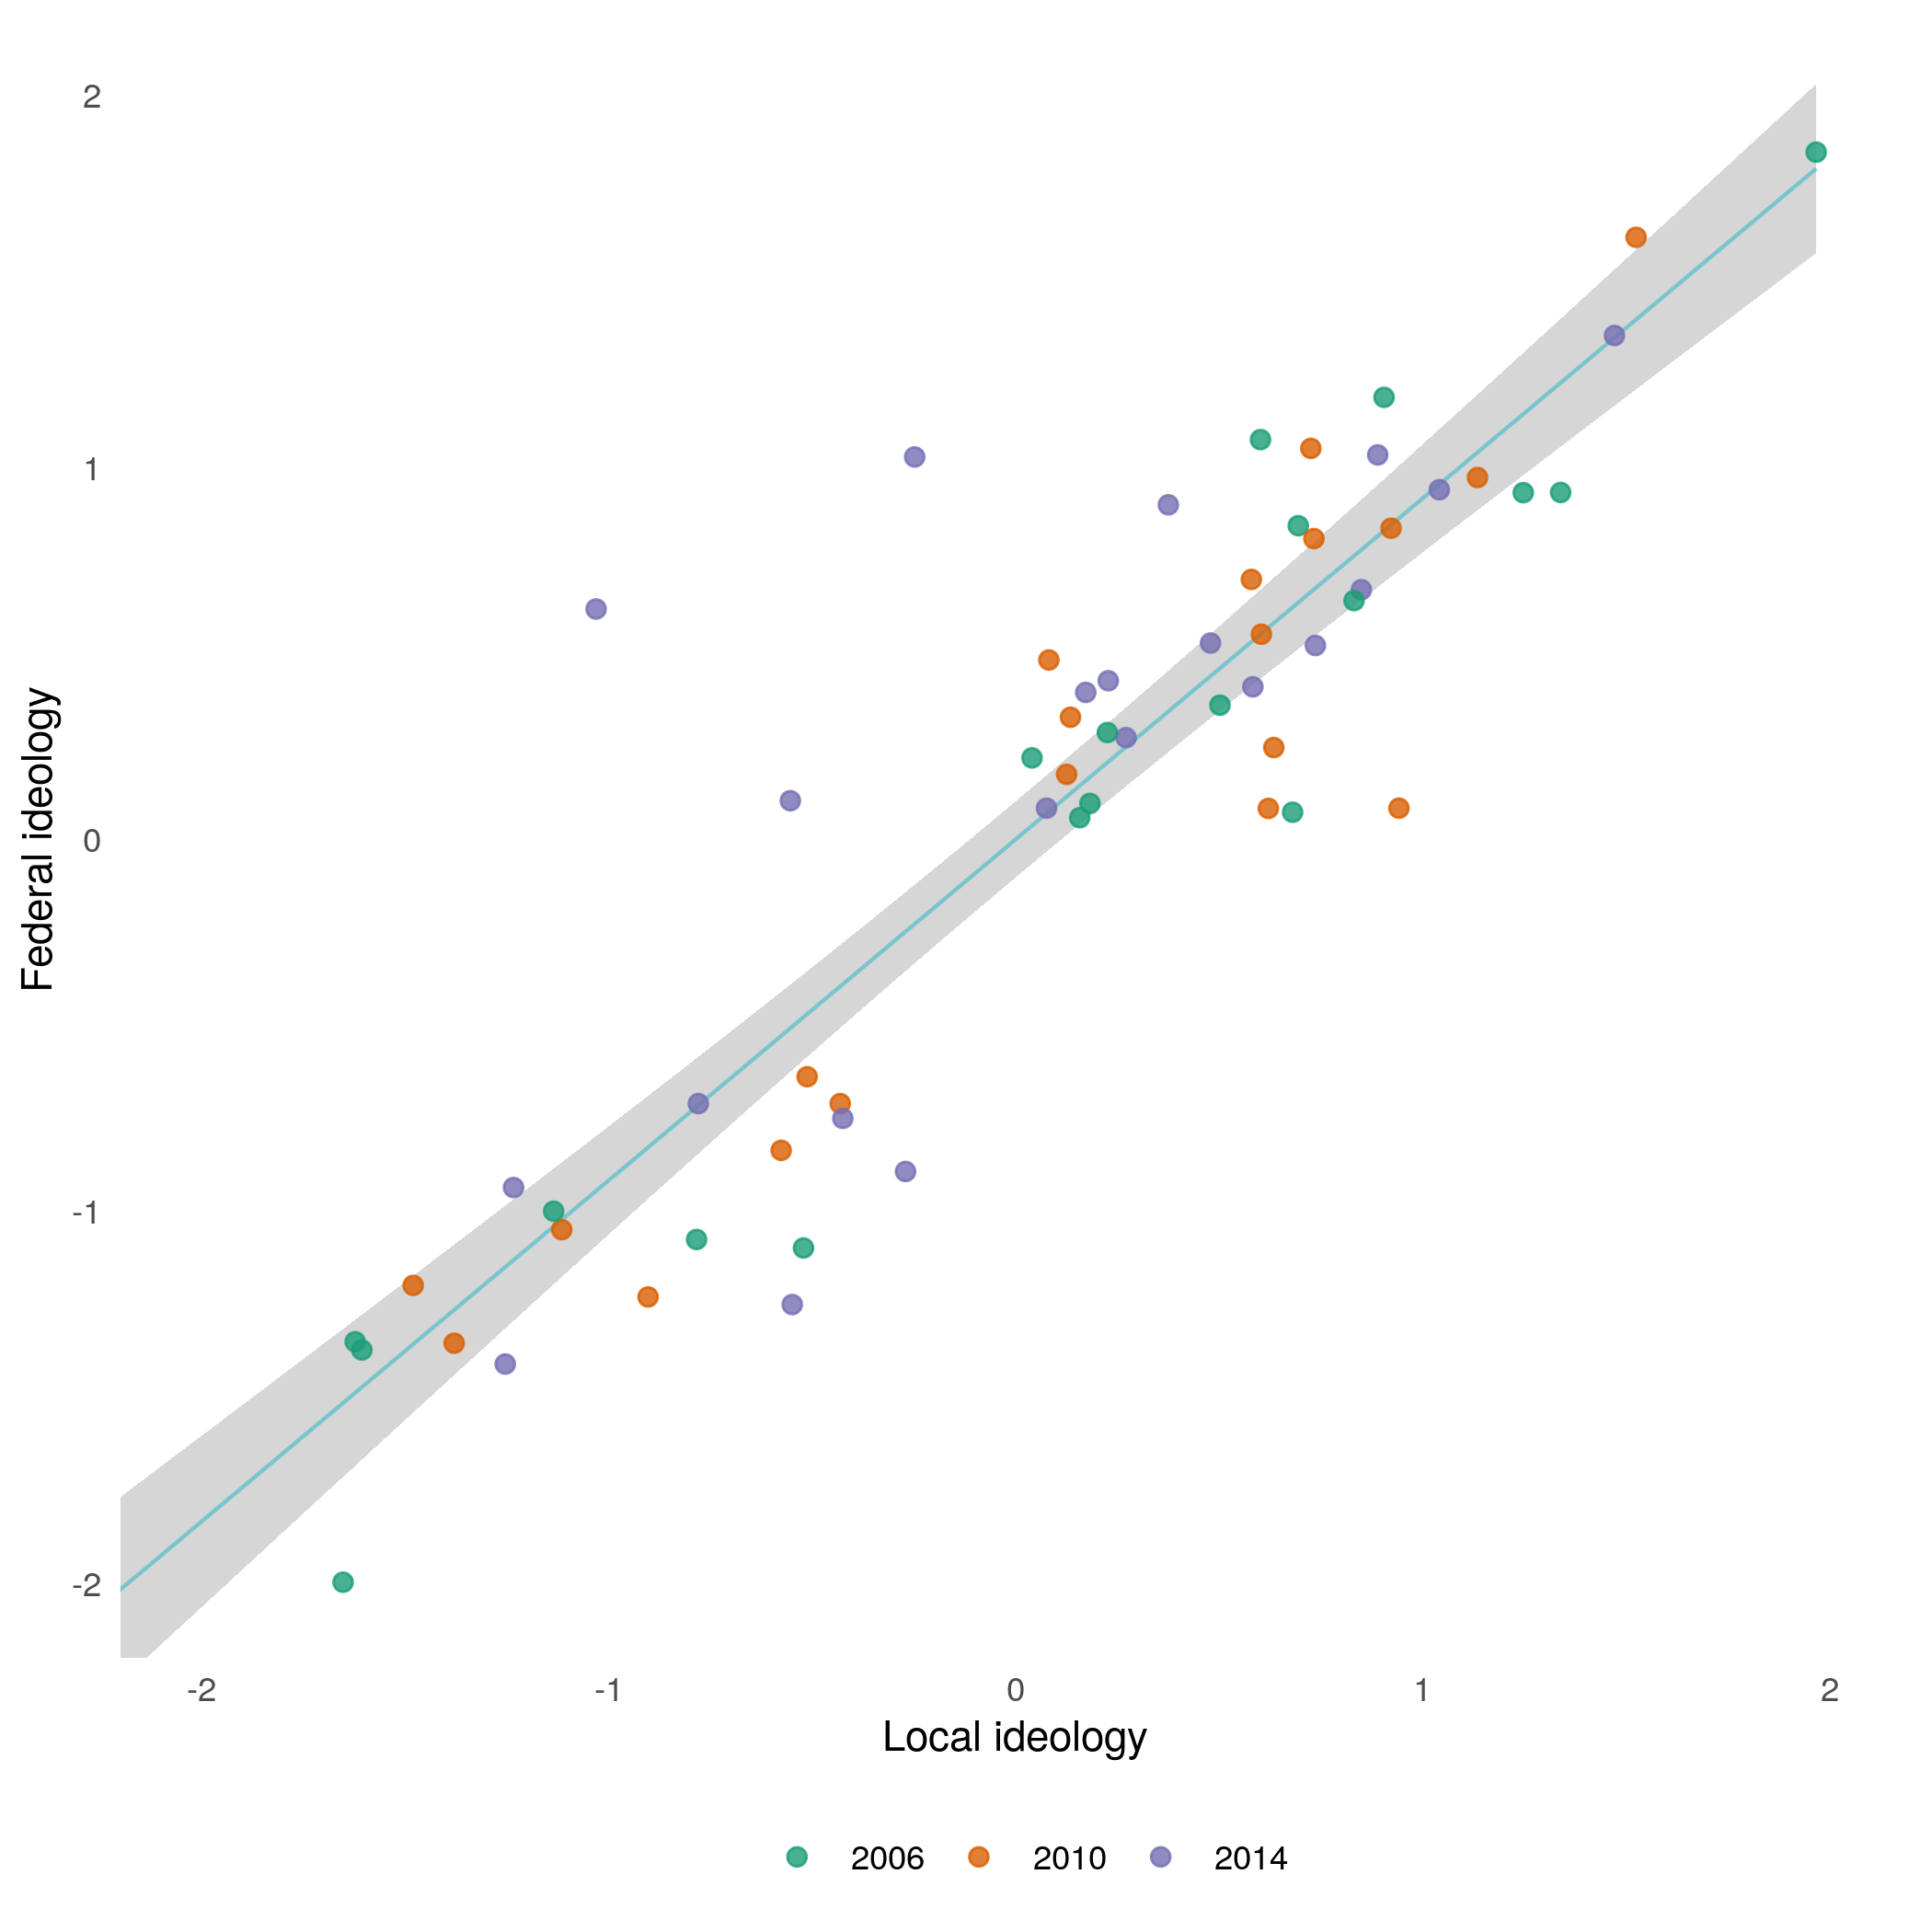
\includegraphics[width=6cm]{\lyxdot ../../Presentation/figs/ideology/reg_ideology.png} &
% 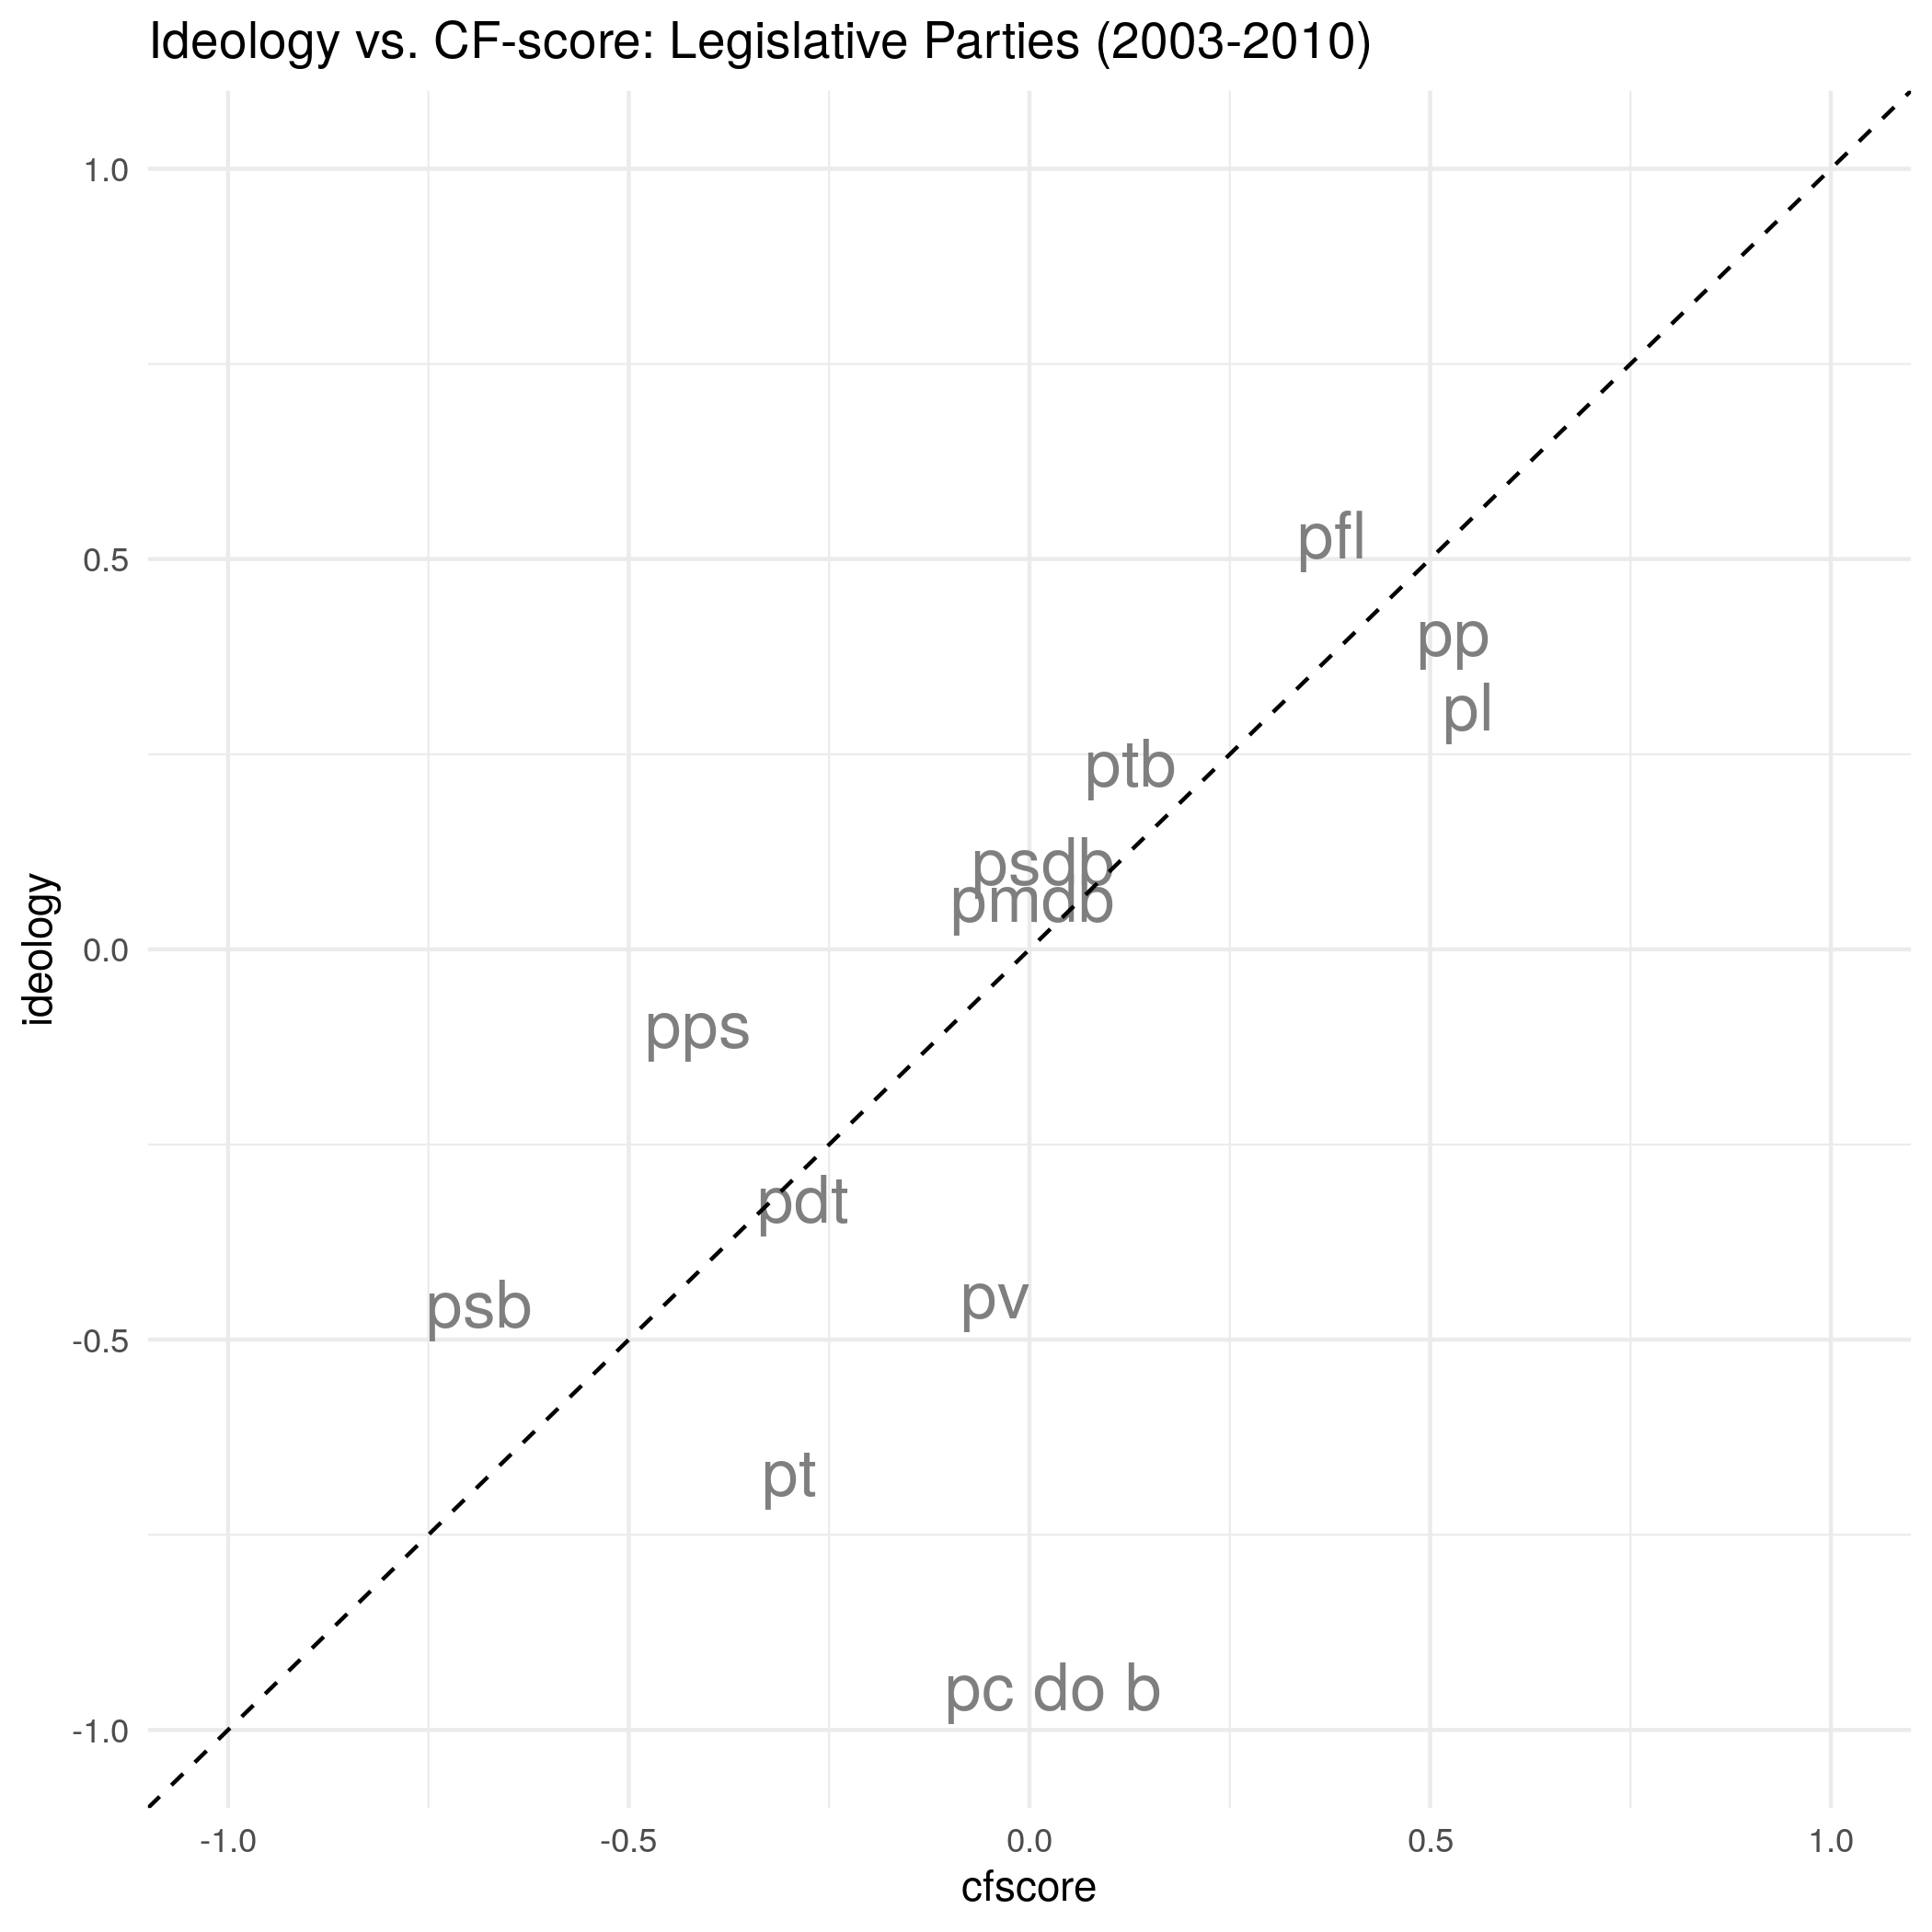
\includegraphics[width=6cm]{\lyxdot ../../Presentation/figs/ideology/ideology_cfscore.png} 
% \end{array}$
% \end{center}
% \caption{Average policy position at the party level, in local and federal-state level races (left) and in the row-call estimation of Power and Zucco (2019) vs. campaign contribution estimations (right).}
%  \label{fig:sanitycheck1}
% \end{figure}

% \begin{figure}[H]
% \begin{center}$
% \begin{array}{cc}
% 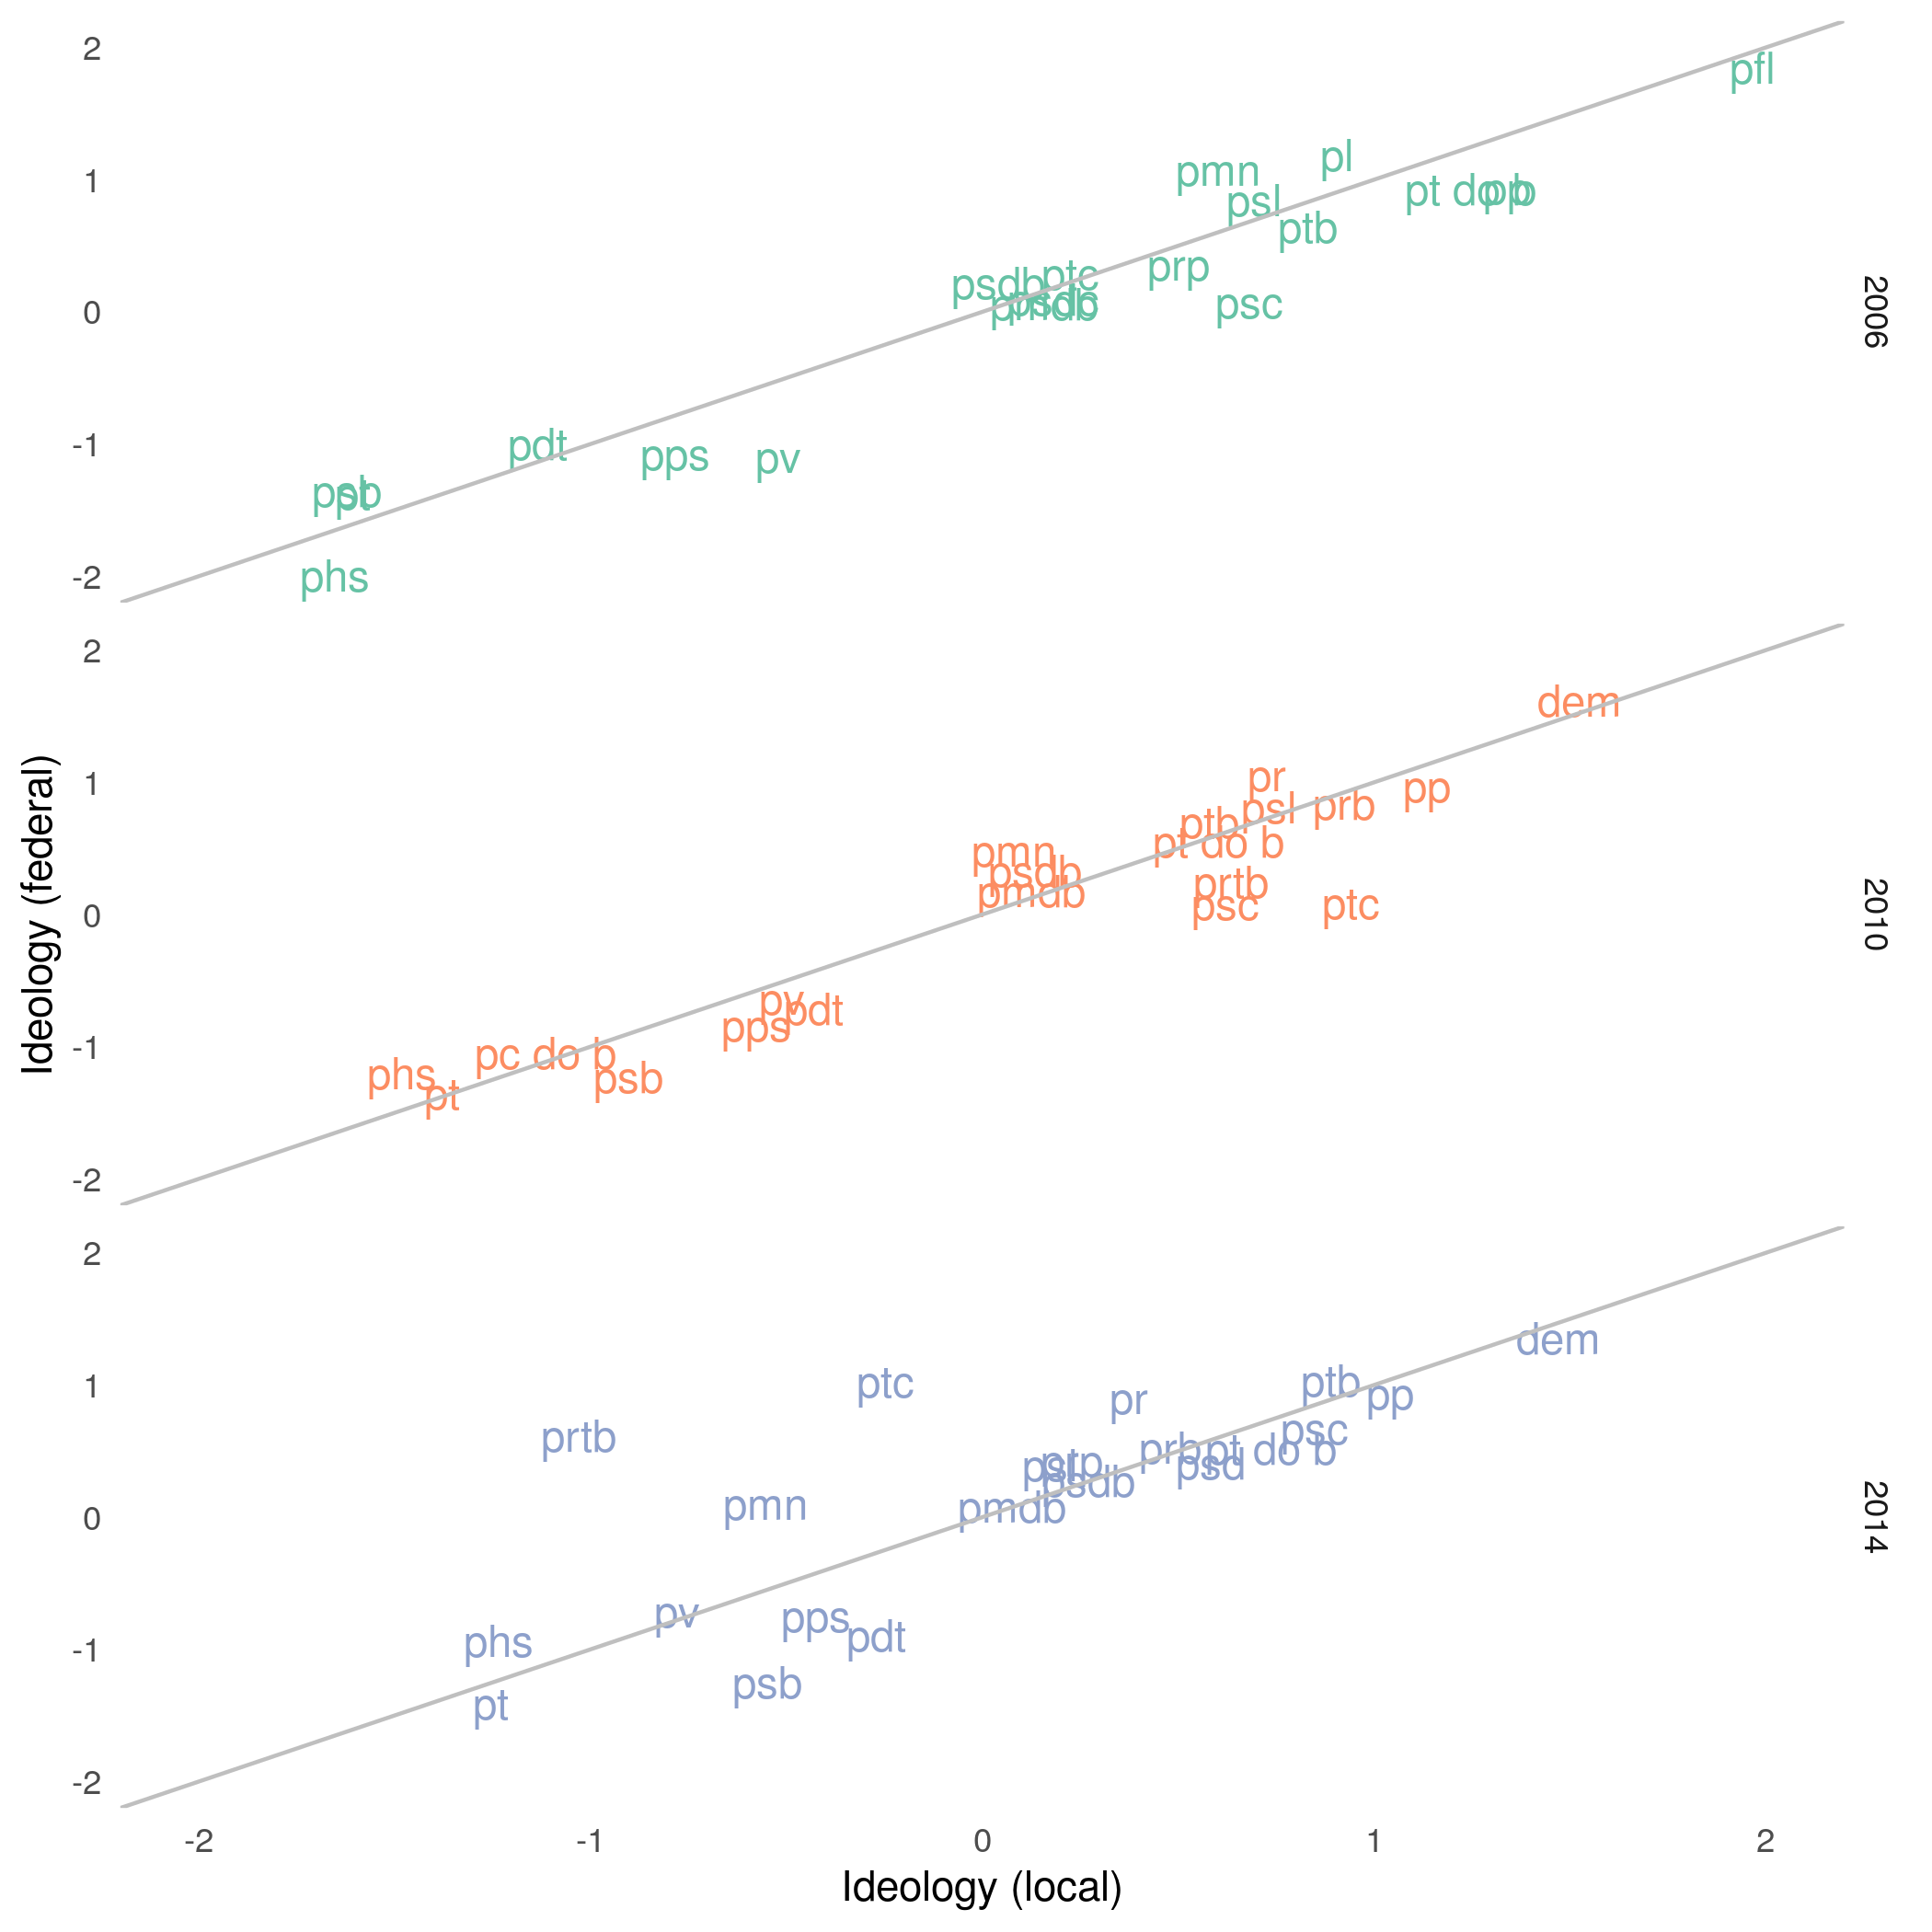
\includegraphics[width=6cm]{\lyxdot /Presentation/figs/ideology/party_ideology_deputy_mayor.png} &
% 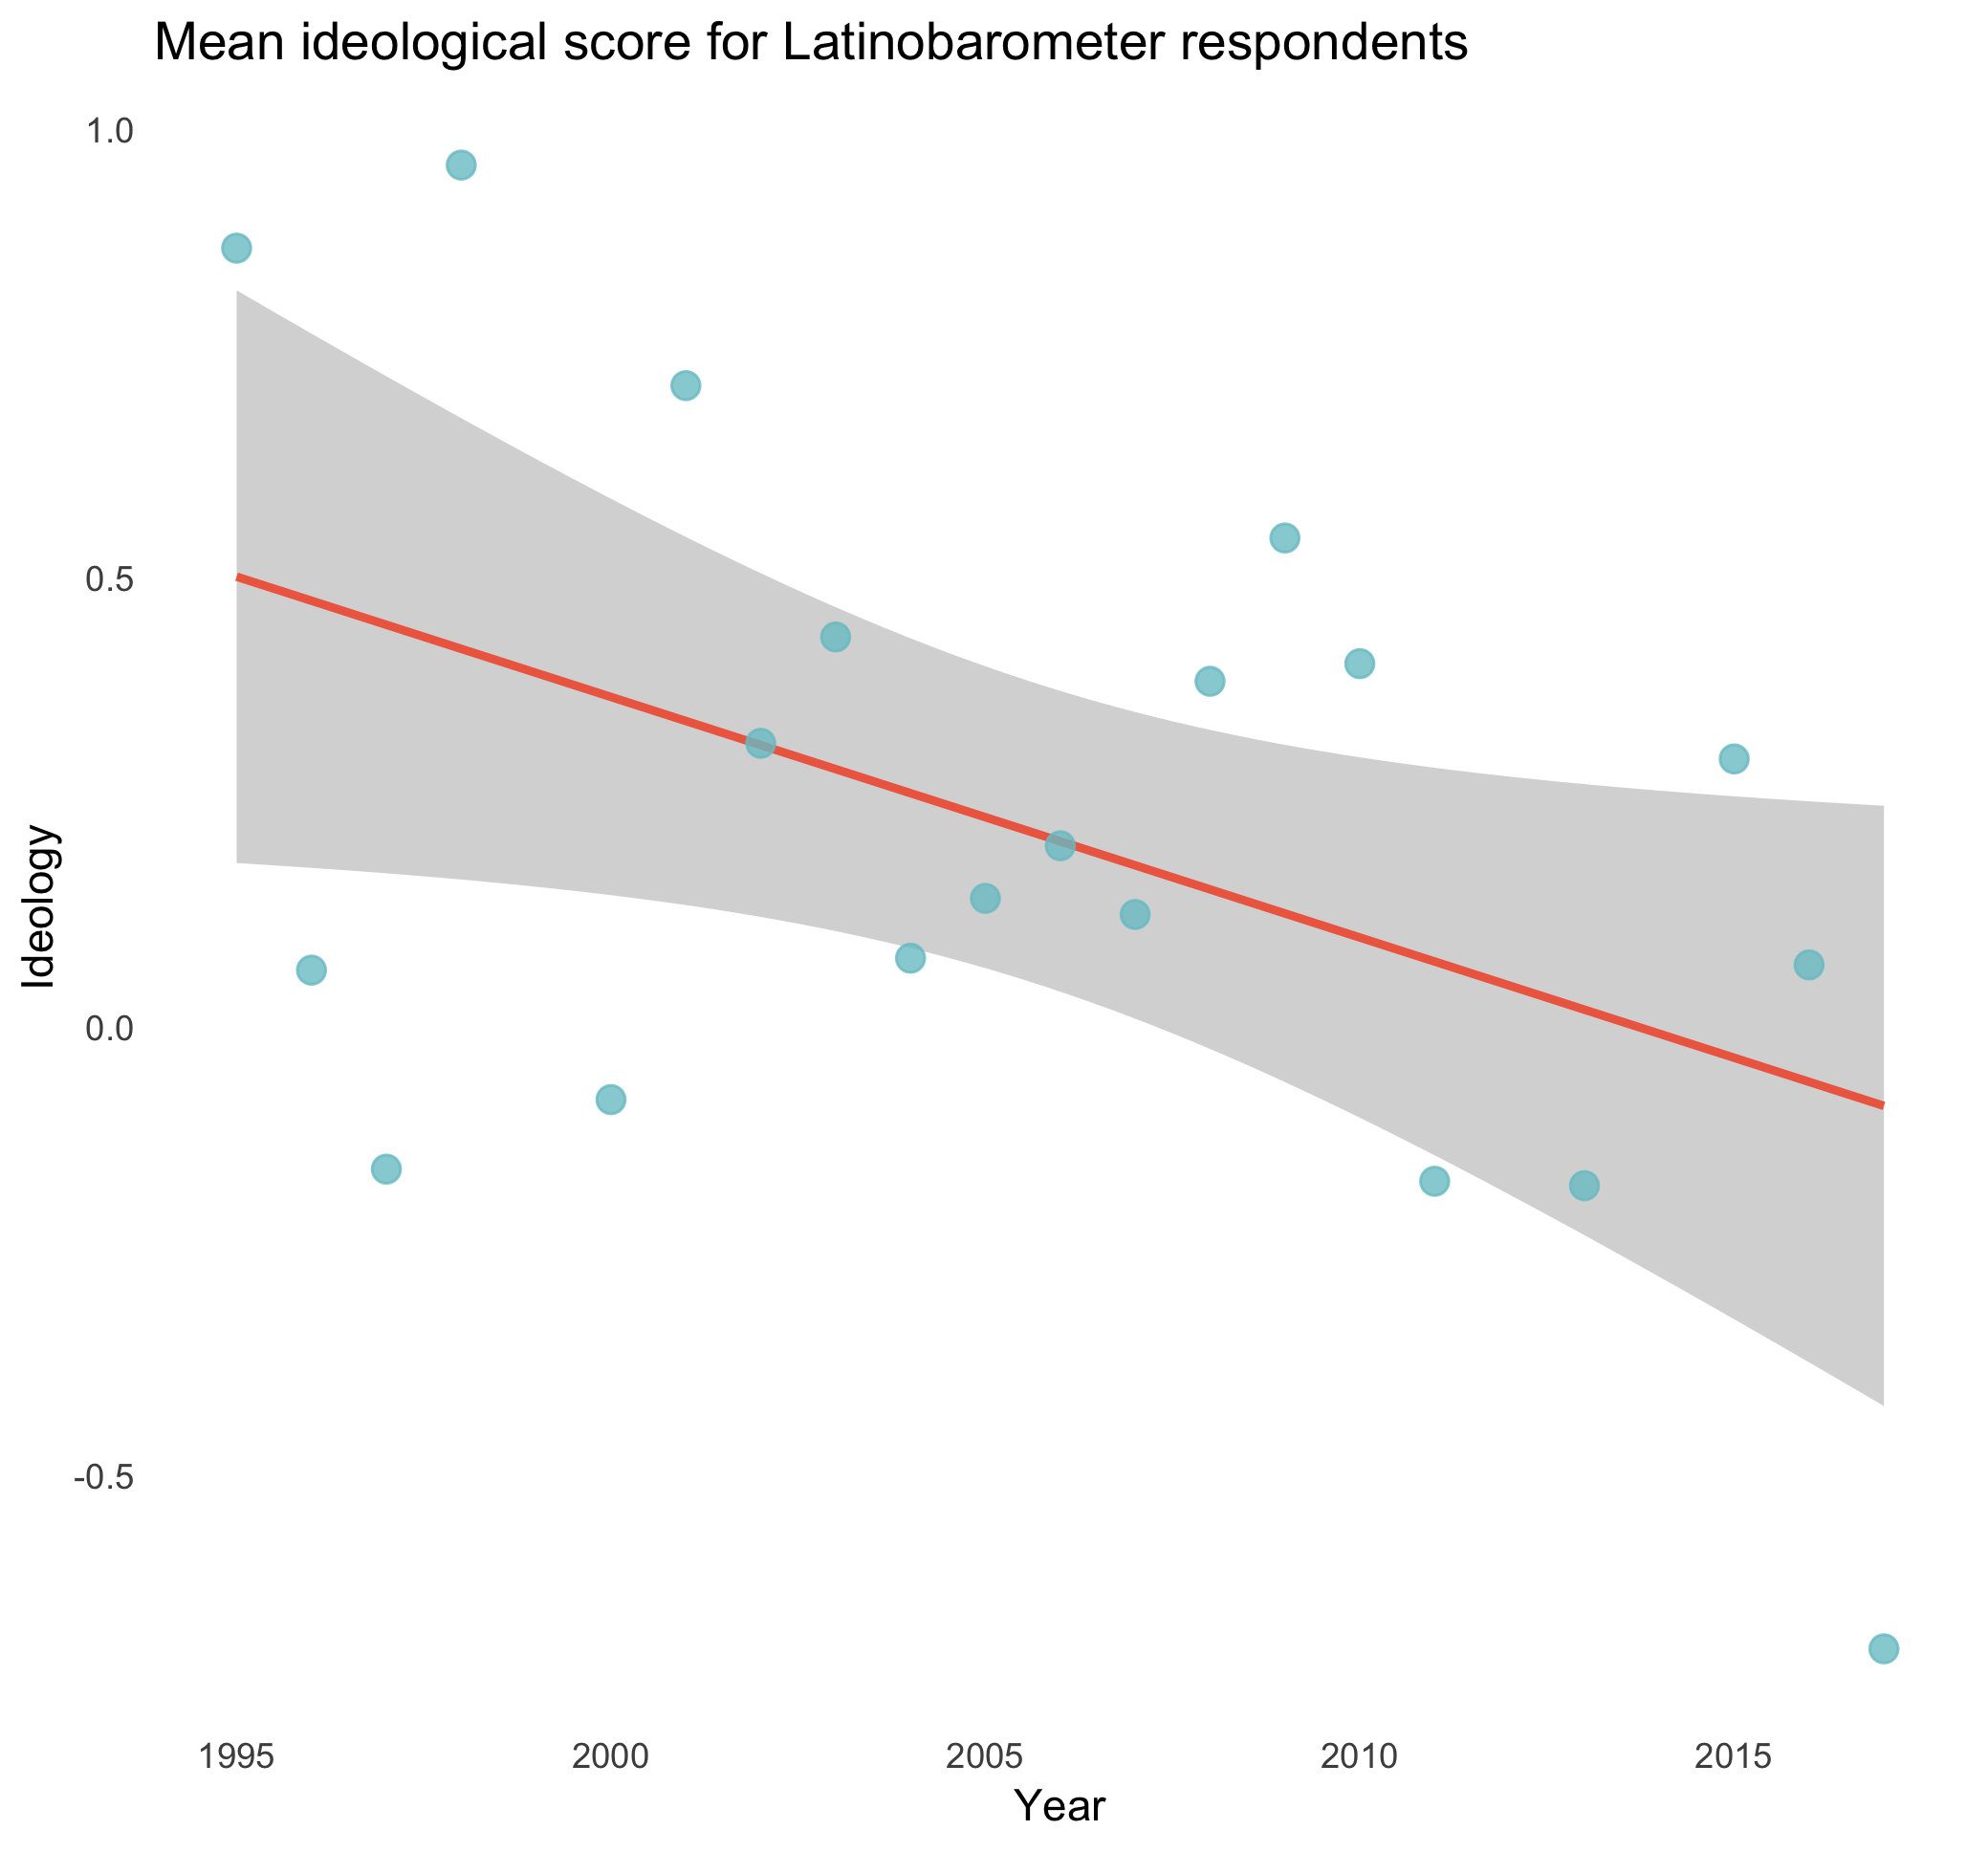
\includegraphics[width=6cm]{\lyxdot /Presentation/figs/ideology/reg_electorate_ideology.png} 
% \end{array}$
% \end{center}
% \caption{\red{CHECK. LABELING IS NOT RIGHT. CAPTION IS POOR TOO}Progressive Movement to the Left of the Ideological Spectrum: in our estimates (left) and in Latinborometer surveys (right). }
%  \label{fig:sanitycheck2}
% \end{figure}

Given the prevalence of corruption in Brazil, we do not take these individual-level campaign donation at face-value. There are well-established concerns regarding corruption in Brazil, in the wake of the largest corruption scandal in Latin America with Operation Carwash. As a result, it is possible that campaign donors may find it worthwhile to donate to candidates in return for public funds or bribes. To address this possibility, we conduct a set of validation exercises to verify if 1) our estimates for candidate ideology are sensitive to excluding largest individual donors and 2) if individual campaign donations are motivated by the possibility of contract allocation. We find no evidence for either hypothesis.

% \begin{figure}[h]
%     \centering
%     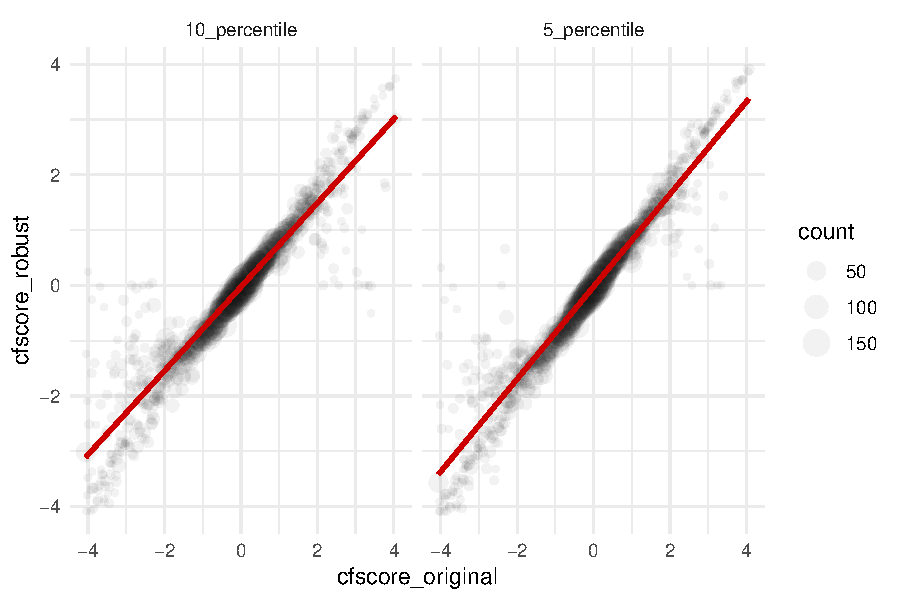
\includegraphics [height=10cm] {./Presentation/figs/ideology/cfscore_robustness.pdf}
%     \caption{\textbf{Policy estimation excluding 5th and 10th percentile.} For each candidate we recompute their policy positions excluding the top 5 and 10 percentile in donors respectively.}
%     \label{fig:cfscore_percentile}
%  \end{figure}

First, we rerun our estimations of candidate policy positions excluding top 5 and 10 percentile donors. Our new estimates have a correlation of 0.9 and 0.847 respectively with the original sample. In figure \ref{fig:cfscore_percentile}, we present a visualization of the new estimates compared to our estimates using the full sample. These findings suggest that our estimates of policy are robust to excluding more generous donors, that may be motivated by other concerns than purely policy preference.

Lastly, to address the concern that campaign donors may be motivated by public contracts, we use the data on public contract allocation by deputado federal provided by \citeasnoun{BoasHidalgoRichardson2014}. We recover the value of contracts disbursed by elected deputados federais in the mandate of 2006-2010 and assess whether it predicts individual campaign donations by the same candidates in the 2010-2014 cycle. Figure \ref{fig:campaign_contract} shows a scatterplot of total logged contracts by candidate and total individual donations received in 2010. We find that there is no significant relationship between these two, suggesting that individual campaign contributors are not motivated by the potential for contract allocations.

%  \begin{figure}[h]
%      \centering
%      \includegraphics[height=10cm]{./Presentation/figs/ideology/validation_contracts_contribution.pdf}
%      \caption{Estimating the assoiation between total contracts disbusrsed and the amount of individual contributors received in the subsequent electoral cycles. Note that the line is flat, suggesting at most a weak relationship between contract disbursements and donations.}
%      \label{fig:campaign_contract}
%  \end{figure} 

\end{document}